% <- percent signs are used to comment
\documentclass[12pt]{article}

%amsmath is a packaged use for typesetting math
%amsfonts is required for special fonts, e.g. blackboard bold (for denoting real numbers, etc.)
\usepackage{amsmath,amsfonts}

%graphicx is required for images
\usepackage{graphicx}

%used for customzing enumarations
\usepackage{enumerate}

%tikz is the package used for trees
\usepackage{tikz}

\usepackage{algo,fullpage,url,amssymb,epsfig,color,xspace}
\usepackage[pdftitle={CS 240 Assignment 0},%
pdfsubject={University of Waterloo, CS 240, Spring 2016},%
pdfauthor={}]{hyperref}

\renewcommand{\thesubsection}{Problem \arabic{subsection}}

%Note: Many of the packages above have other uses beyond those used in this document

%this marks the beginning of the document. Everything before this is called the Preamble.
\begin{document}
%marks the end of the title section
\begin{center}
{\Large\bf University of Waterloo}\\
\vspace{3mm}
{\Large\bf CS240, Spring 2016}\\
\vspace{2mm}
{\Large\bf Assigment 0}\\
\vspace{3mm}
\textbf{Wednesday, May 11}
\end{center}

\definecolor{care}{rgb}{0,0,0}
\def\question#1{\item[\bf #1.]}
\def\part#1{\item[\bf #1)]}
\newcommand{\pc}[1]{\mbox{\textbf{#1}}} % pseudocode

\section*{Problem 1 - Assignment Guidelines}

\begin{enumerate}[a)]
    \item If an assignment question asks you to design an algorithm, in addition
to describing/writing the pseudocode for the algorithm, you must explain the main idea if it's helpful, give a proof or argument of correctness if it is not immediately obvious, and include an analysis (usually, of the running time).

    \item For programming questions, the input can be read using standard input stream (\texttt{std::cin}) and the output can be written to the standard output stream (\texttt{std::cout}).
\end{enumerate}

\section*{Problem 2 - Mathematics}

Let P(n) by our inductive statement.

\begin{align*}
P(n): \sum_{i = 1}^{n} i &= \frac{n(n+1)}{2}
\end{align*}

\begin{enumerate}[1)]
\item{{\bf Base Case}: We verify that P(1) is true where P(1) is the statement
\begin{align*}
P(1): \sum_{i = 1}^{1} i &= \frac{1(1+1)}{2} \\
 &= 1
\end{align*}
}

\item{{\bf Inductive Hypothesis}: We assume P(k) is true for some integer k \geq 1.

\begin{align*}
P(k): \sum_{i = 1}^{k} i &= \frac{k(k+1)}{2} 
\end{align*}
}

\item{{\bf Inductive Conclusion}: Now we show that the statement P(k+1) is true.

\begin{align*}
    \sum_{i = 1}^{k} i + (k+1) &= \frac{(k)(k+1)}{2} + (k+1) \qquad (inductive\enspace hypothesis) \\
    \sum_{i = 1}^{k+1} i &= \frac{(k)(k+1)}{2} + \frac{2(k+1)}{2} \\
    P(k+1): \sum_{i = 1}^{k+1} i &= \frac{(k+1)((k+1)+1)}{2}
    \end{align*}
}

The result is true for n = k+1, and so holds for all n by the Principle of Mathematical
Induction.

\end{enumerate}

\section*{Problem 3 - Trees}

\begin{center}\begin{tikzpicture}[
  level distance=45 pt,
  every node/.style={circle,draw},
  level 1/.style={sibling distance=200 pt},
  level 2/.style={sibling distance=100 pt},
  level 3/.style={sibling distance=60 pt}
]
  \node {M$_0$}
    child {node {F$_0$}
      child {node {C$_0$}
        child {node {A$_0$}}
        child[missing]
      }
      child {node {I$_0$}
        child {node {G$_0$}}
        child[missing]
      }
    }
    child {node {T$_0$}
      child {node {Q$_0$}}
      child {node {W$_0$}
        child {node {U$_0$}}
        child[missing]
      }
    };
\end{tikzpicture}\end{center}

\section*{Problem 4 - Plots}

\begin{center}
\begin{tikzpicture}
		\draw[thick,]  (0,15) -- (0,0) node[left] {0};
		\draw[thick,]  (0,0) -- (15,0) node[below] {15};
		\draw[thick,]  (15,15) -- (15,0) node[left] {};
		\draw[thick,]  (15,15) -- (0,15) node[left] {15};
		\draw[thick,]  (6, 0) -- (6,15) node[left] {};
		\draw[thick,]  (0, 6) -- (6,6) node[left] {};
		\draw[thick,]  (6, 4) -- (15,4) node[left] {};
		\draw[thick,]  (2, 6) -- (2, 15) node[left] {};
		\draw[thick,]  (3, 0) -- (3, 6) node[left] {};
		\draw[thick,]  (9, 0) -- (9, 4) node[left] {};
		\draw[dashed,]  (2, 0.5) -- (6.5, 0.5) node[left] {};
		\draw[dashed,]  (2, 7) -- (6.5, 7) node[left] {};
		\draw[dashed,]  (2, 0.5) -- (2, 7) node[left] {};
		\draw[dashed,]  (6.5, 0.5) -- (6.5, 7) node[left] {};
		 
		\fill (6, 2) circle[radius=2.5pt] node[left]{(6, 2)};
		\fill (4, 6) circle[radius=2.5pt] node[below]{(4, 6)};
		\fill (3, 5) circle[radius=2.5pt] node[right]{(3, 5)};
		\fill (0, 3) circle[radius=2.5pt] node[right]{(0, 3)};
		\fill (2, 9) circle[radius=2.5pt] node[right]{(2, 9)};
		\fill (1, 7) circle[radius=2.5pt] node[below]{(1, 7)};
		\fill (10, 4) circle[radius=2.5pt] node[below]{(10, 4)};
		\fill (9, 1) circle[radius=2.5pt] node[right]{(9, 1)};
		\fill (8, 0) circle[radius=2.5pt] node[above]{(8, 0)};
		\fill (7, 8) circle[radius=2.5pt] node[right]{(7, 8)};
		\fill (15, 10) circle[radius=2.5pt] node[left]{(15, 10)};

\end{tikzpicture}
\end{center}

\section*{Problem 5 - Tables}

\begin{tabular}{ | l || r  | r | c | c |} \hline
  Animal's Name & Avg. Weight & Longevity & Avg. Temperature & Conservation Status  \\ \hline
   Polar Bear & 350-700kg & 25 years & 37$^{\circ}$C  & Vulnerable \\ \hline
   Cheetah & 21-72kg & 10-12 years & 38.3$^{\circ}$C & Vulnerable \\ \hline
\end{tabular}

\section*{Problem 6 - Images}

\begin{figure}
\begin{center}
        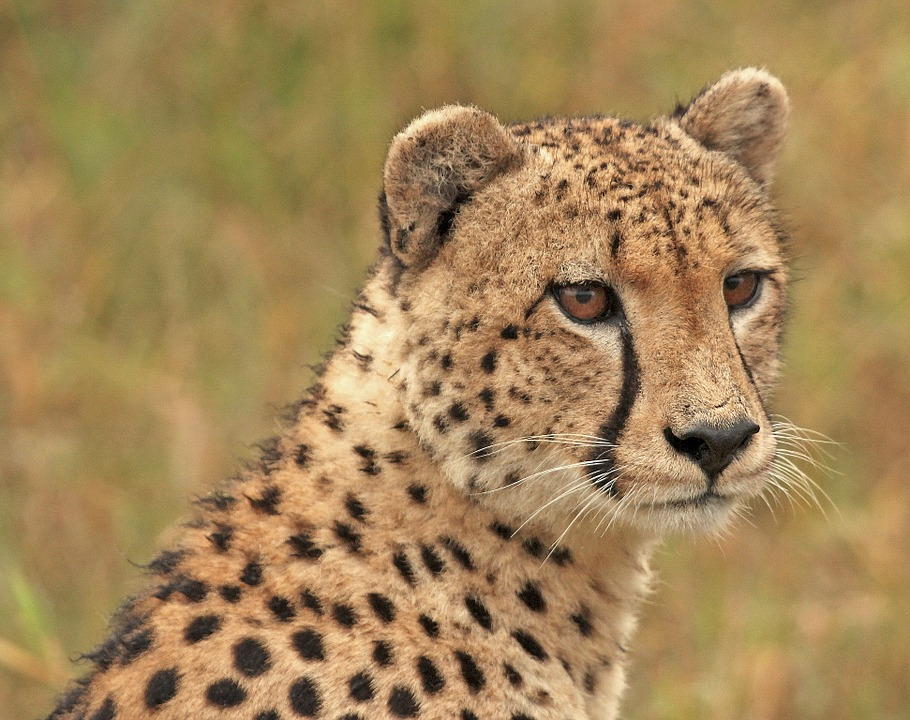
\includegraphics[scale=0.2]{cheetah.jpg}
\end{center}
\caption{\label{figcaption} Cheetah}
\end{figure}

\end{document}